\documentclass{article}
\usepackage{graphicx}
\usepackage{fancyhdr}
\usepackage{geometry}

% Page layout
\geometry{a4paper, margin=1in}
\pagestyle{fancy}
\fancyhf{}
\rhead{\textbf{ArduinoNanoCircuit Unplugged Lab}}
\lhead{}
\rfoot{\thepage}

% Font
\renewcommand{\familydefault}{\sfdefault}

\begin{document}

\title{ArduinoNanoCircuit Unplugged Lab}
\author{}
\date{}
% \maketitle

\newpage
\section*{Blinking LED}
\begin{minipage}{\textwidth}
Connect an LED to \texttt{pin 3}. Blinks the LED on and off.
\end{minipage}
\begin{figure}[h!]
\centering
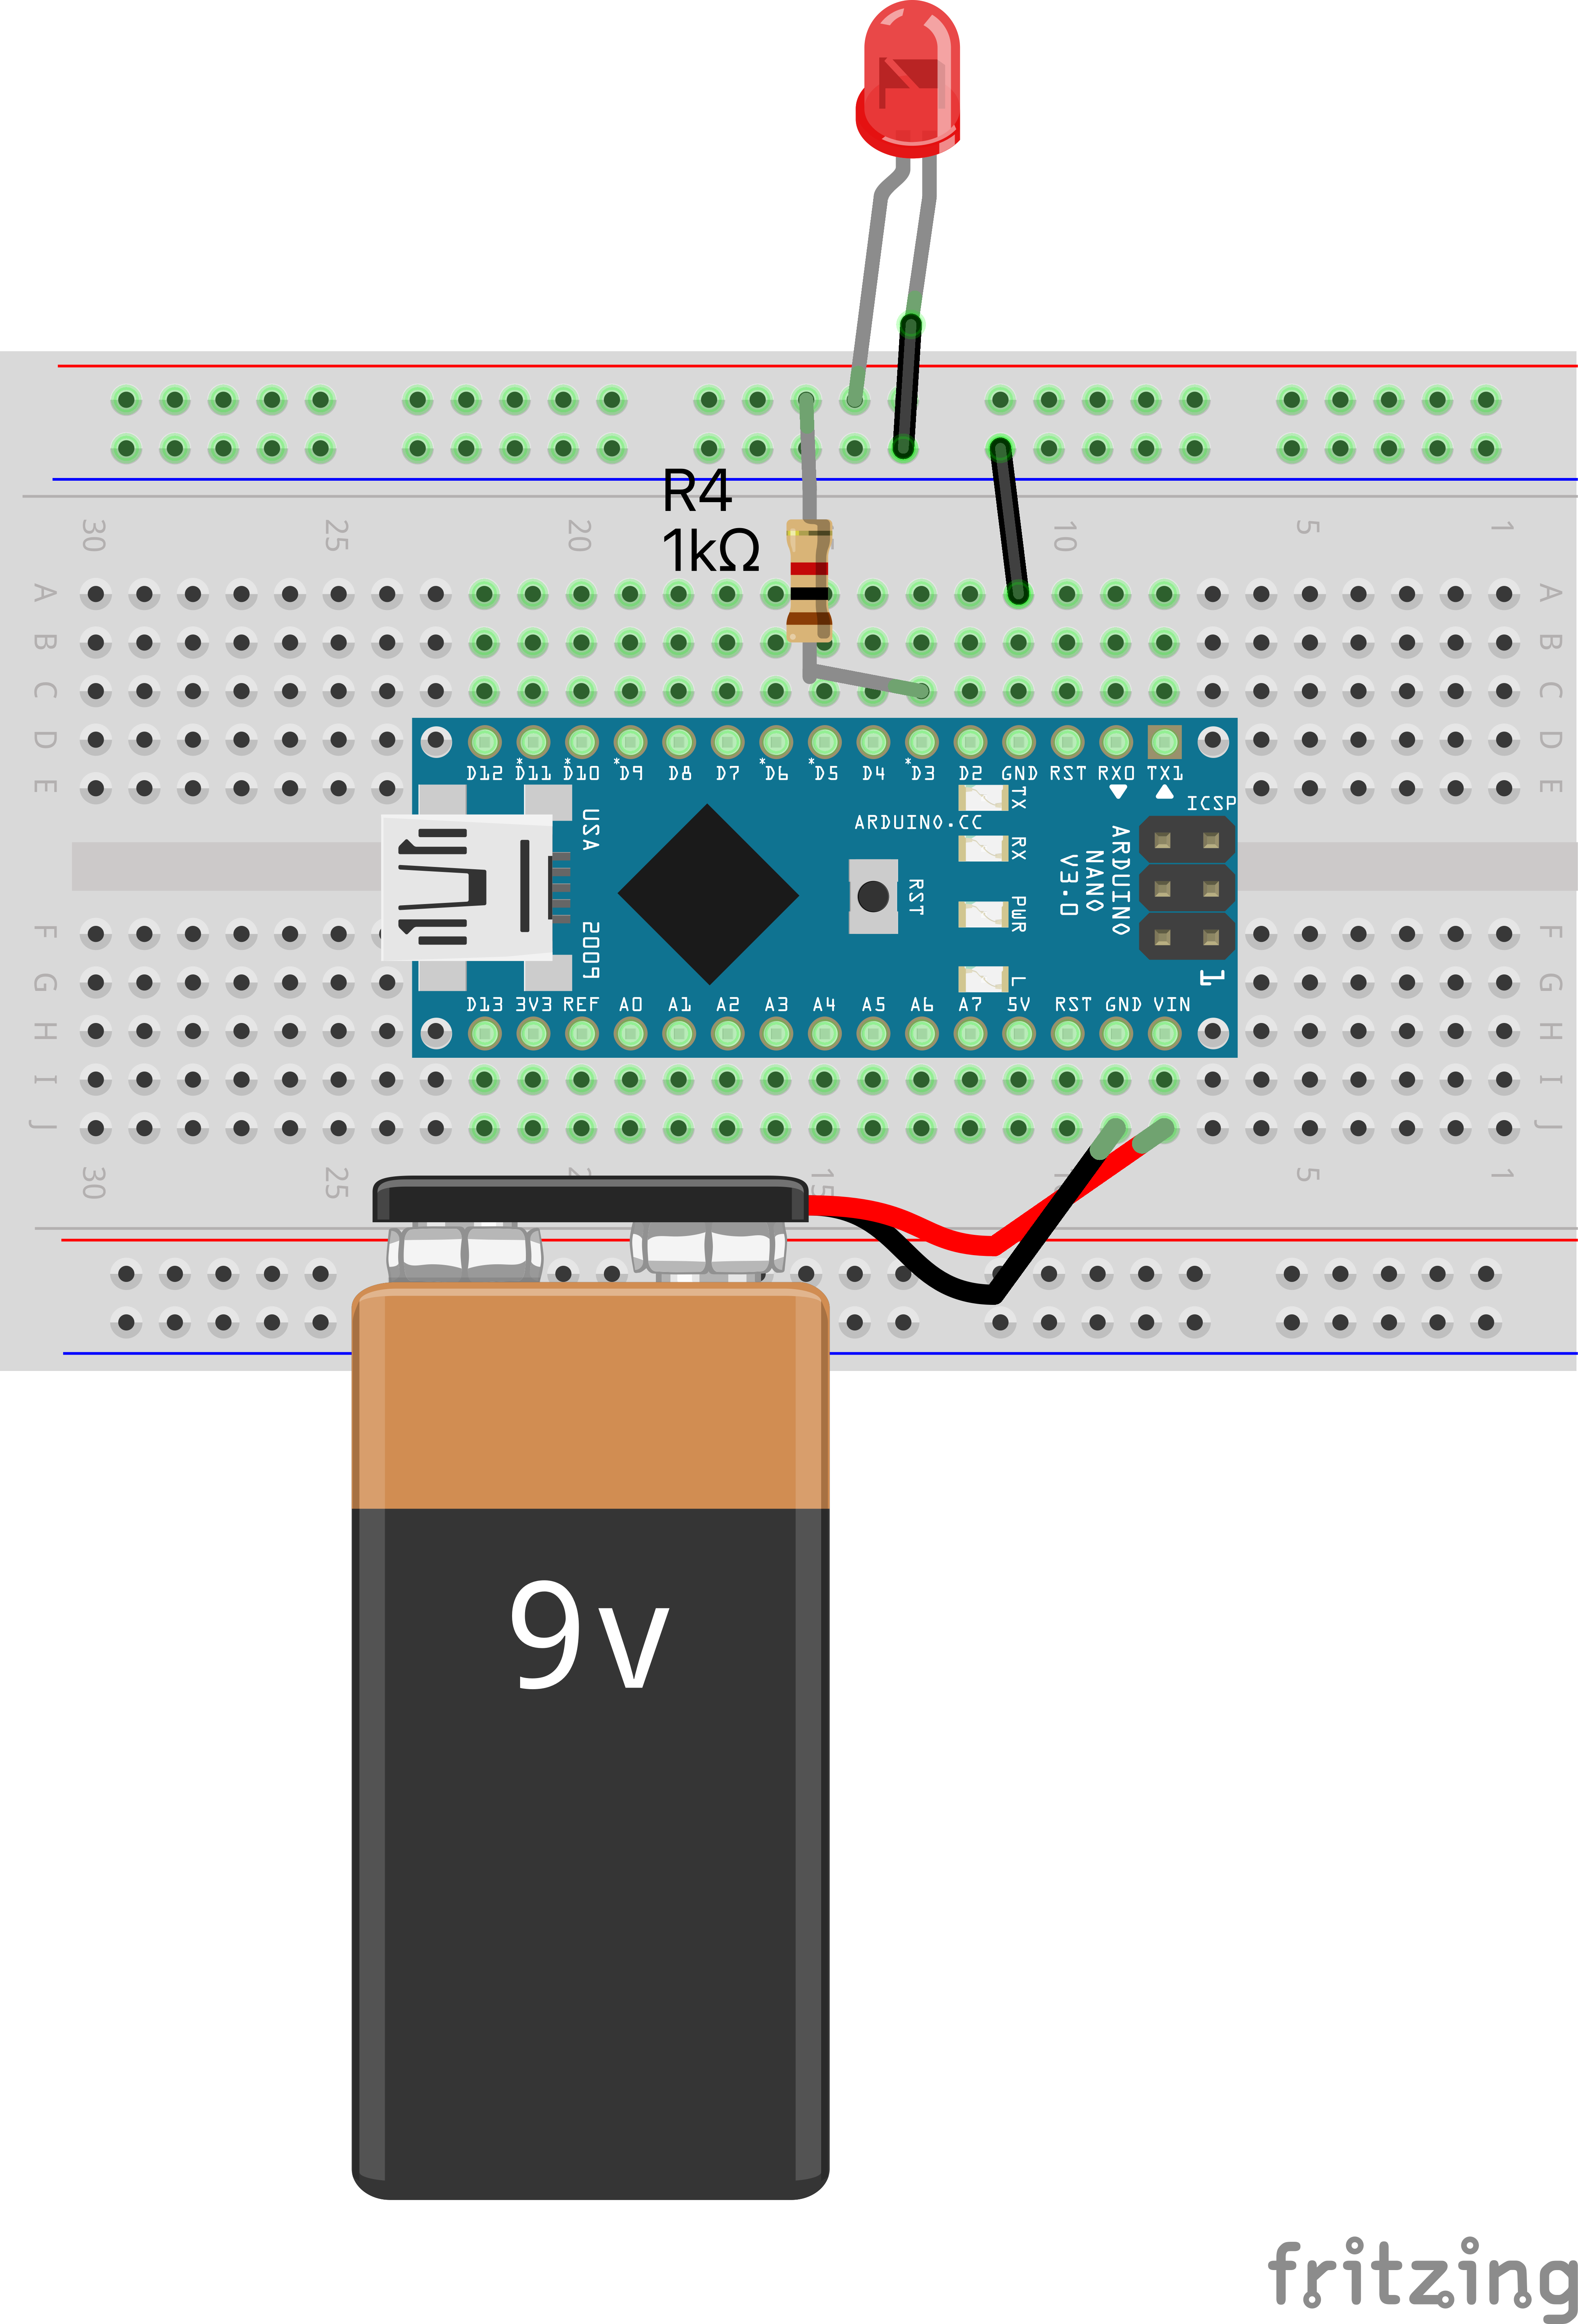
\includegraphics[width=0.8\textwidth]{led_basic_nano_bb.png}
\end{figure}
\newpage

\section*{Fading LED}
\begin{minipage}{\textwidth}
Connect an LED to \texttt{pin 5}. Gradually change the LED brightness.
\end{minipage}
\begin{figure}[h!]
\centering
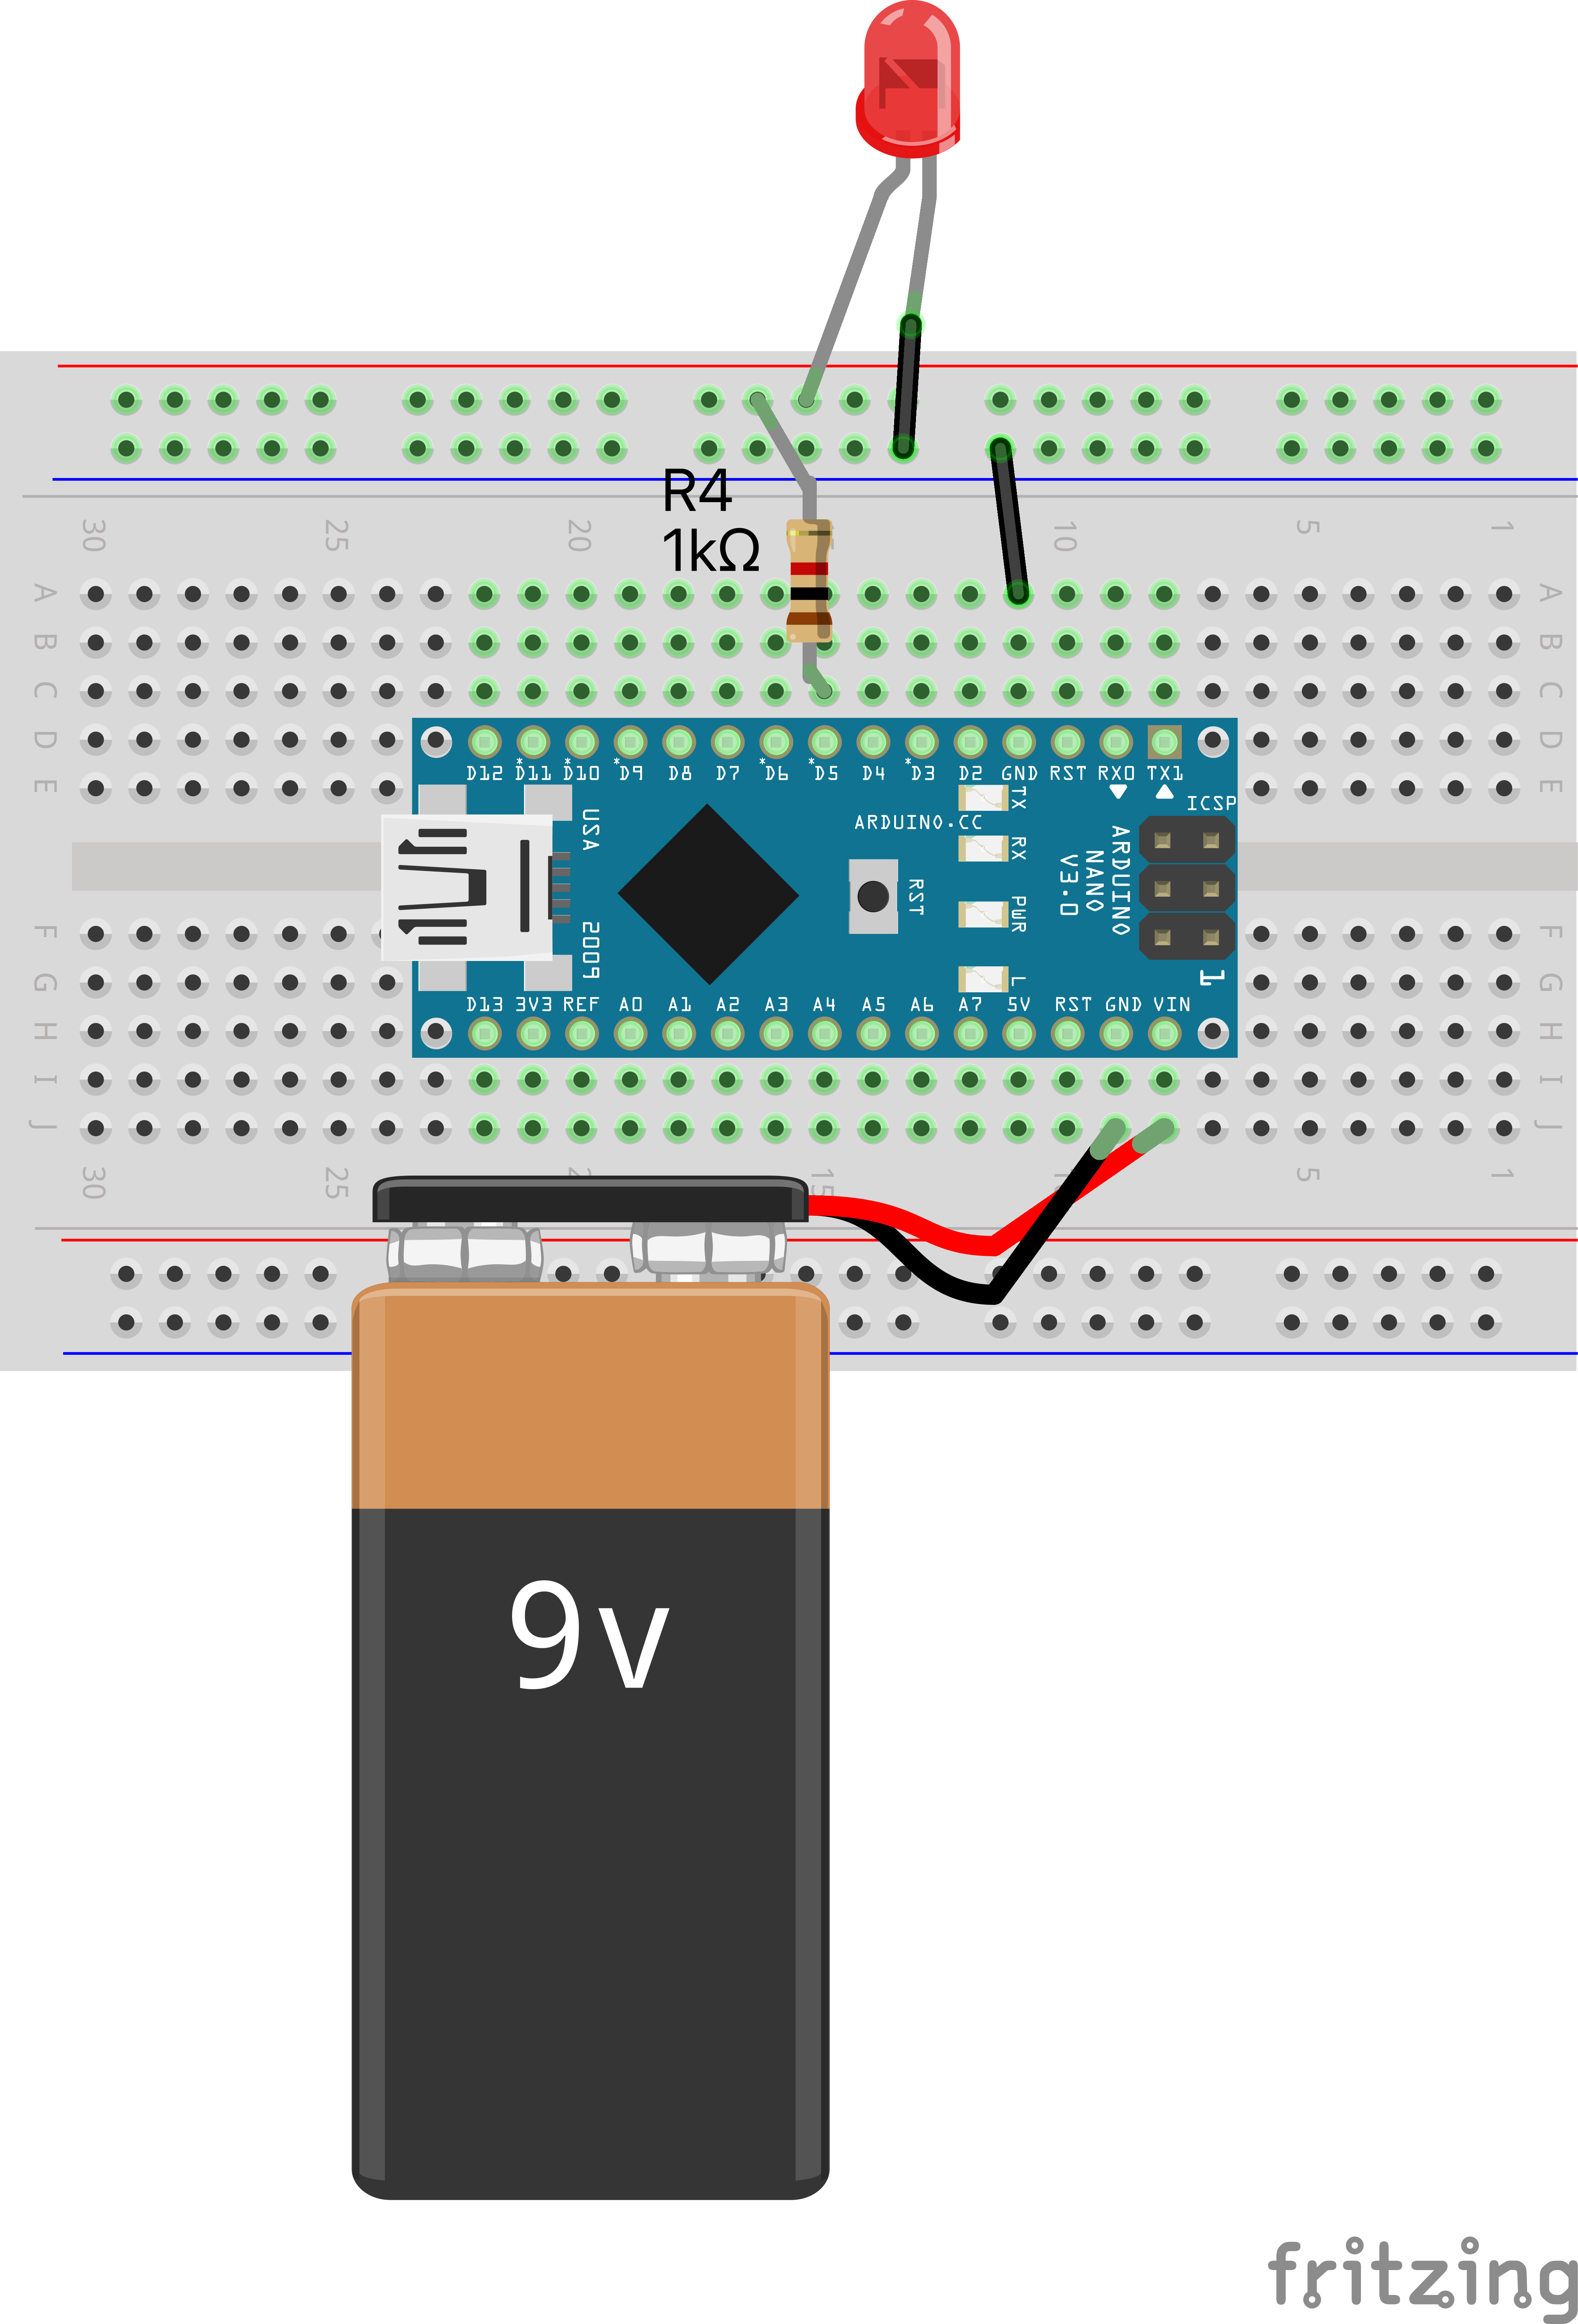
\includegraphics[width=0.8\textwidth]{fade_nano_bb.png}
\end{figure}
\newpage

\section*{DC Motor}
\begin{minipage}{\textwidth}
Connect a DC motor to \texttt{pin 9}. Controls the motor speed and direction.
\end{minipage}
\begin{figure}[h!]
\centering
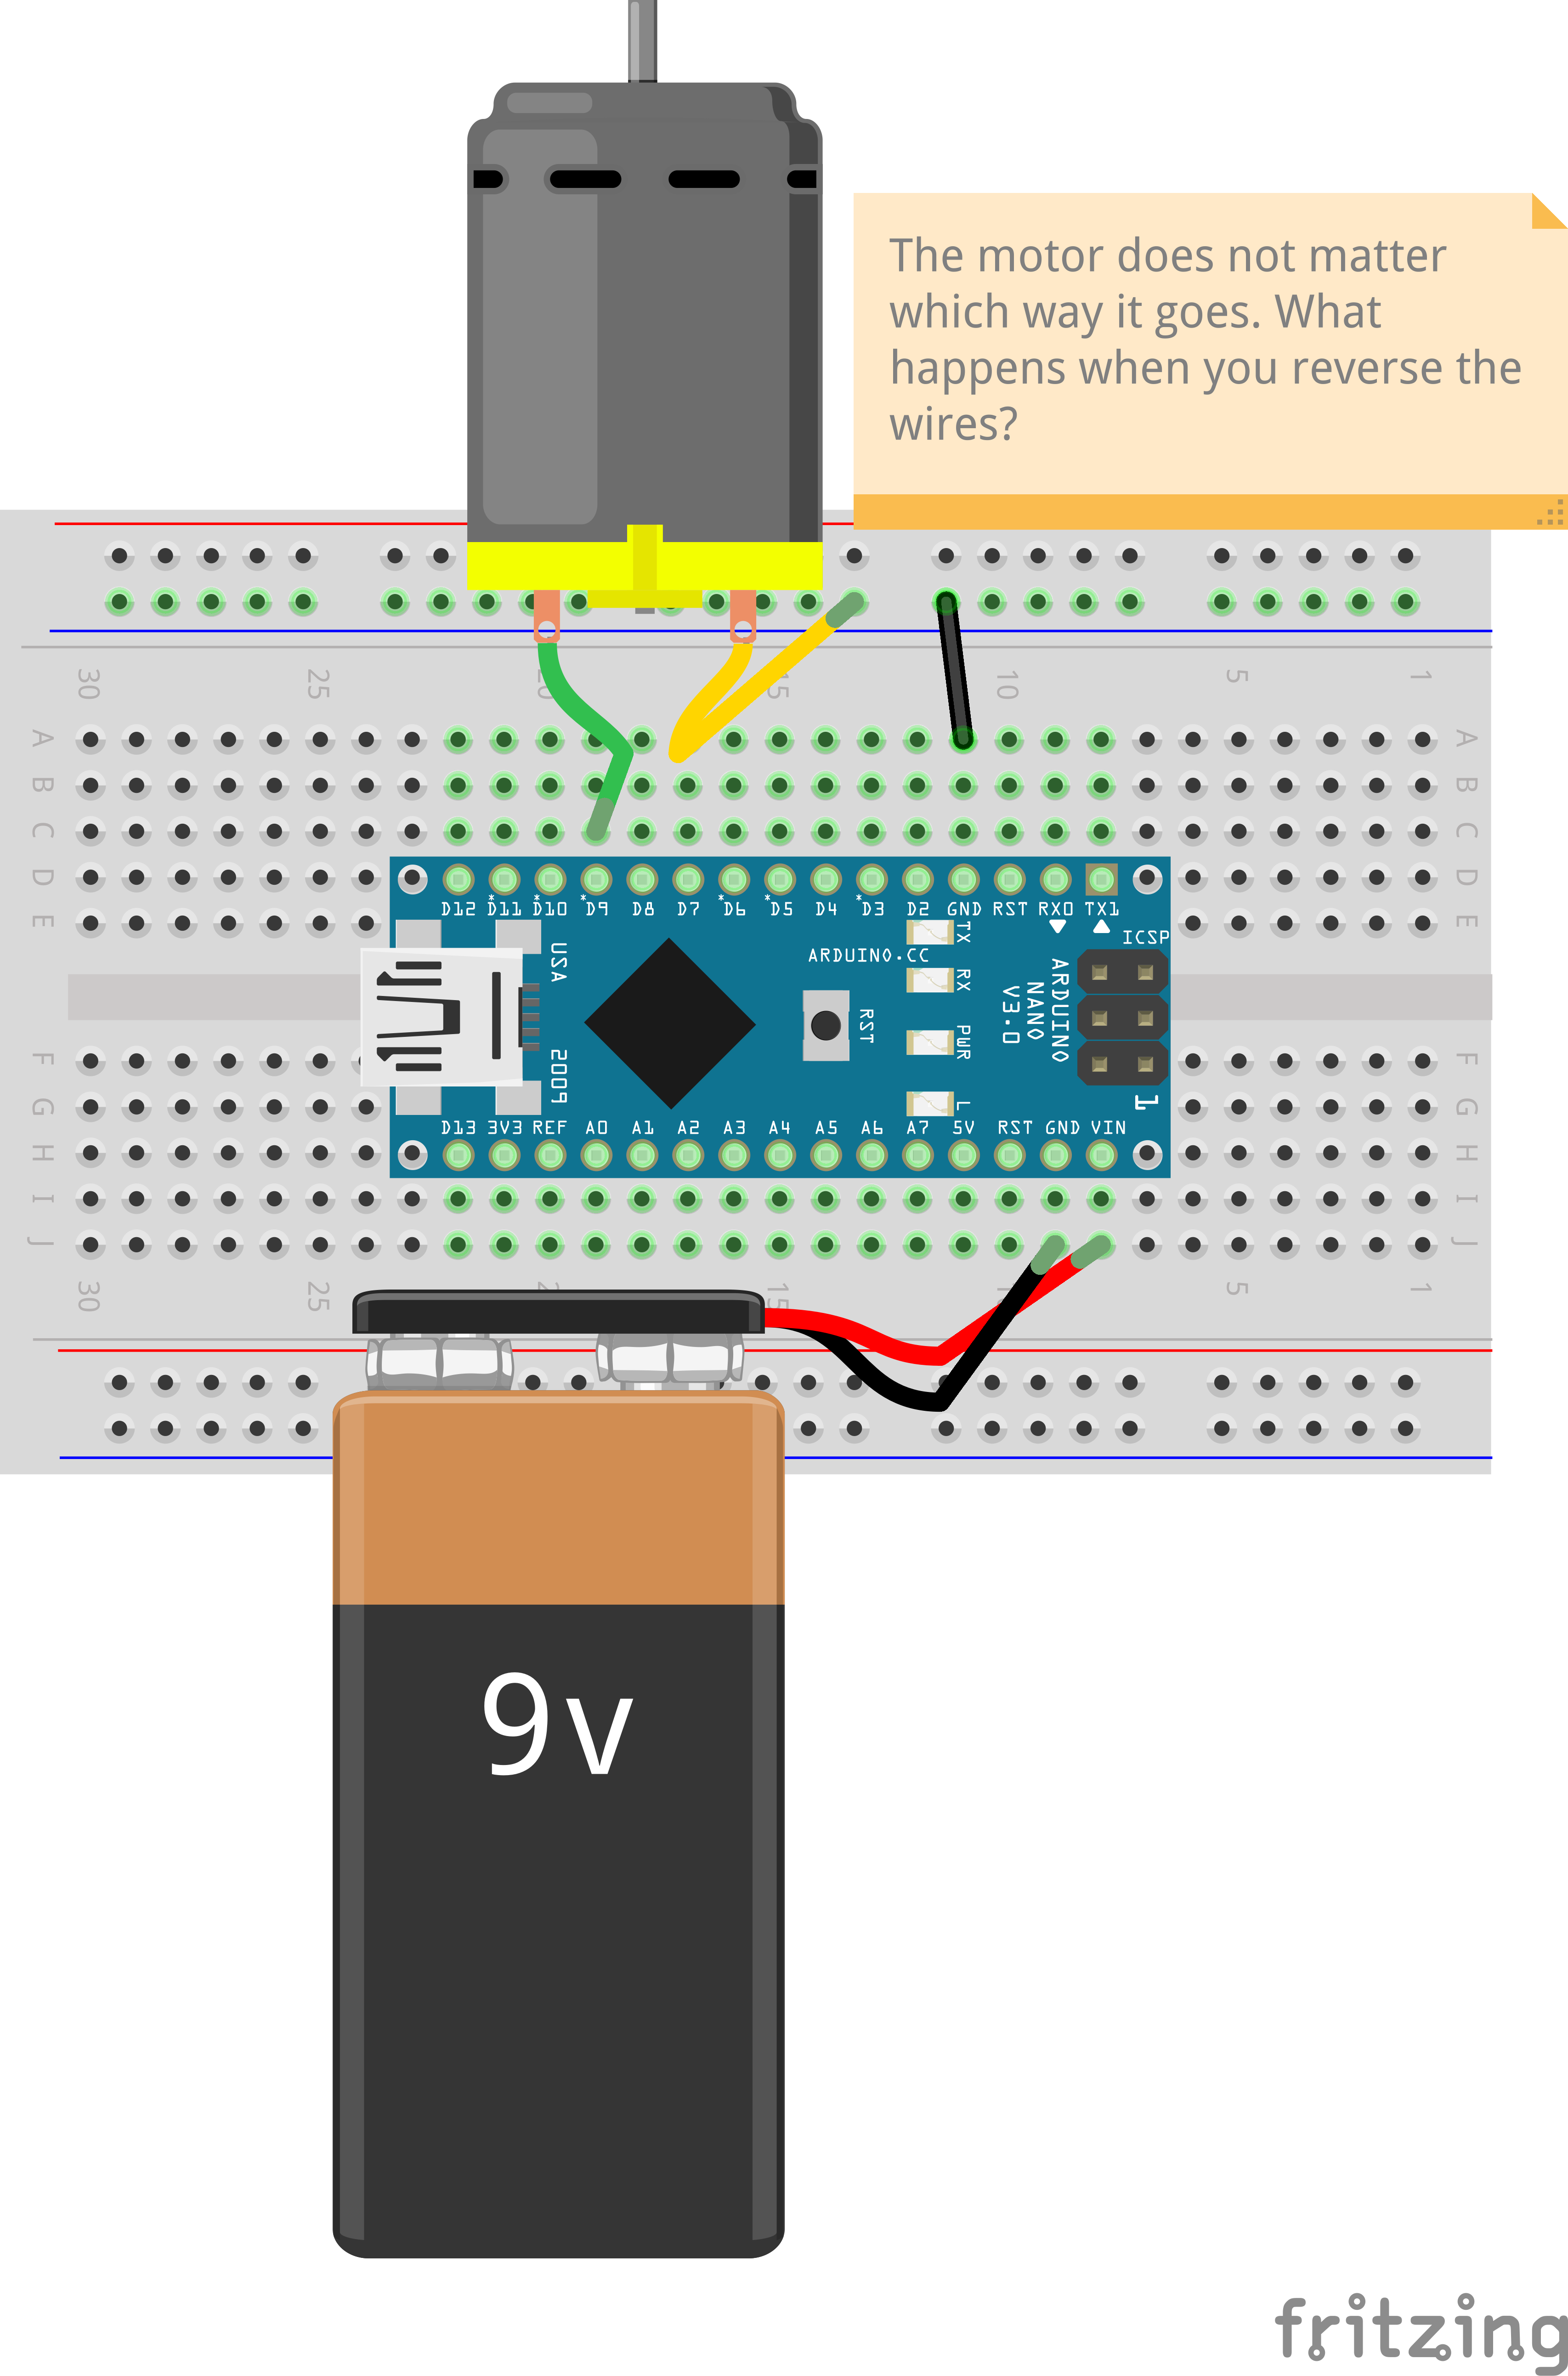
\includegraphics[width=0.8\textwidth]{motor_nano_bb.png}
\end{figure}
\newpage

\section*{Slide Switch Control}
\begin{minipage}{\textwidth}
Connect a slide switch to \texttt{pin 2}. Connect an LED to \texttt{pin 8}. Toggle an LED with the switch.
\end{minipage}
\begin{figure}[h!]
\centering
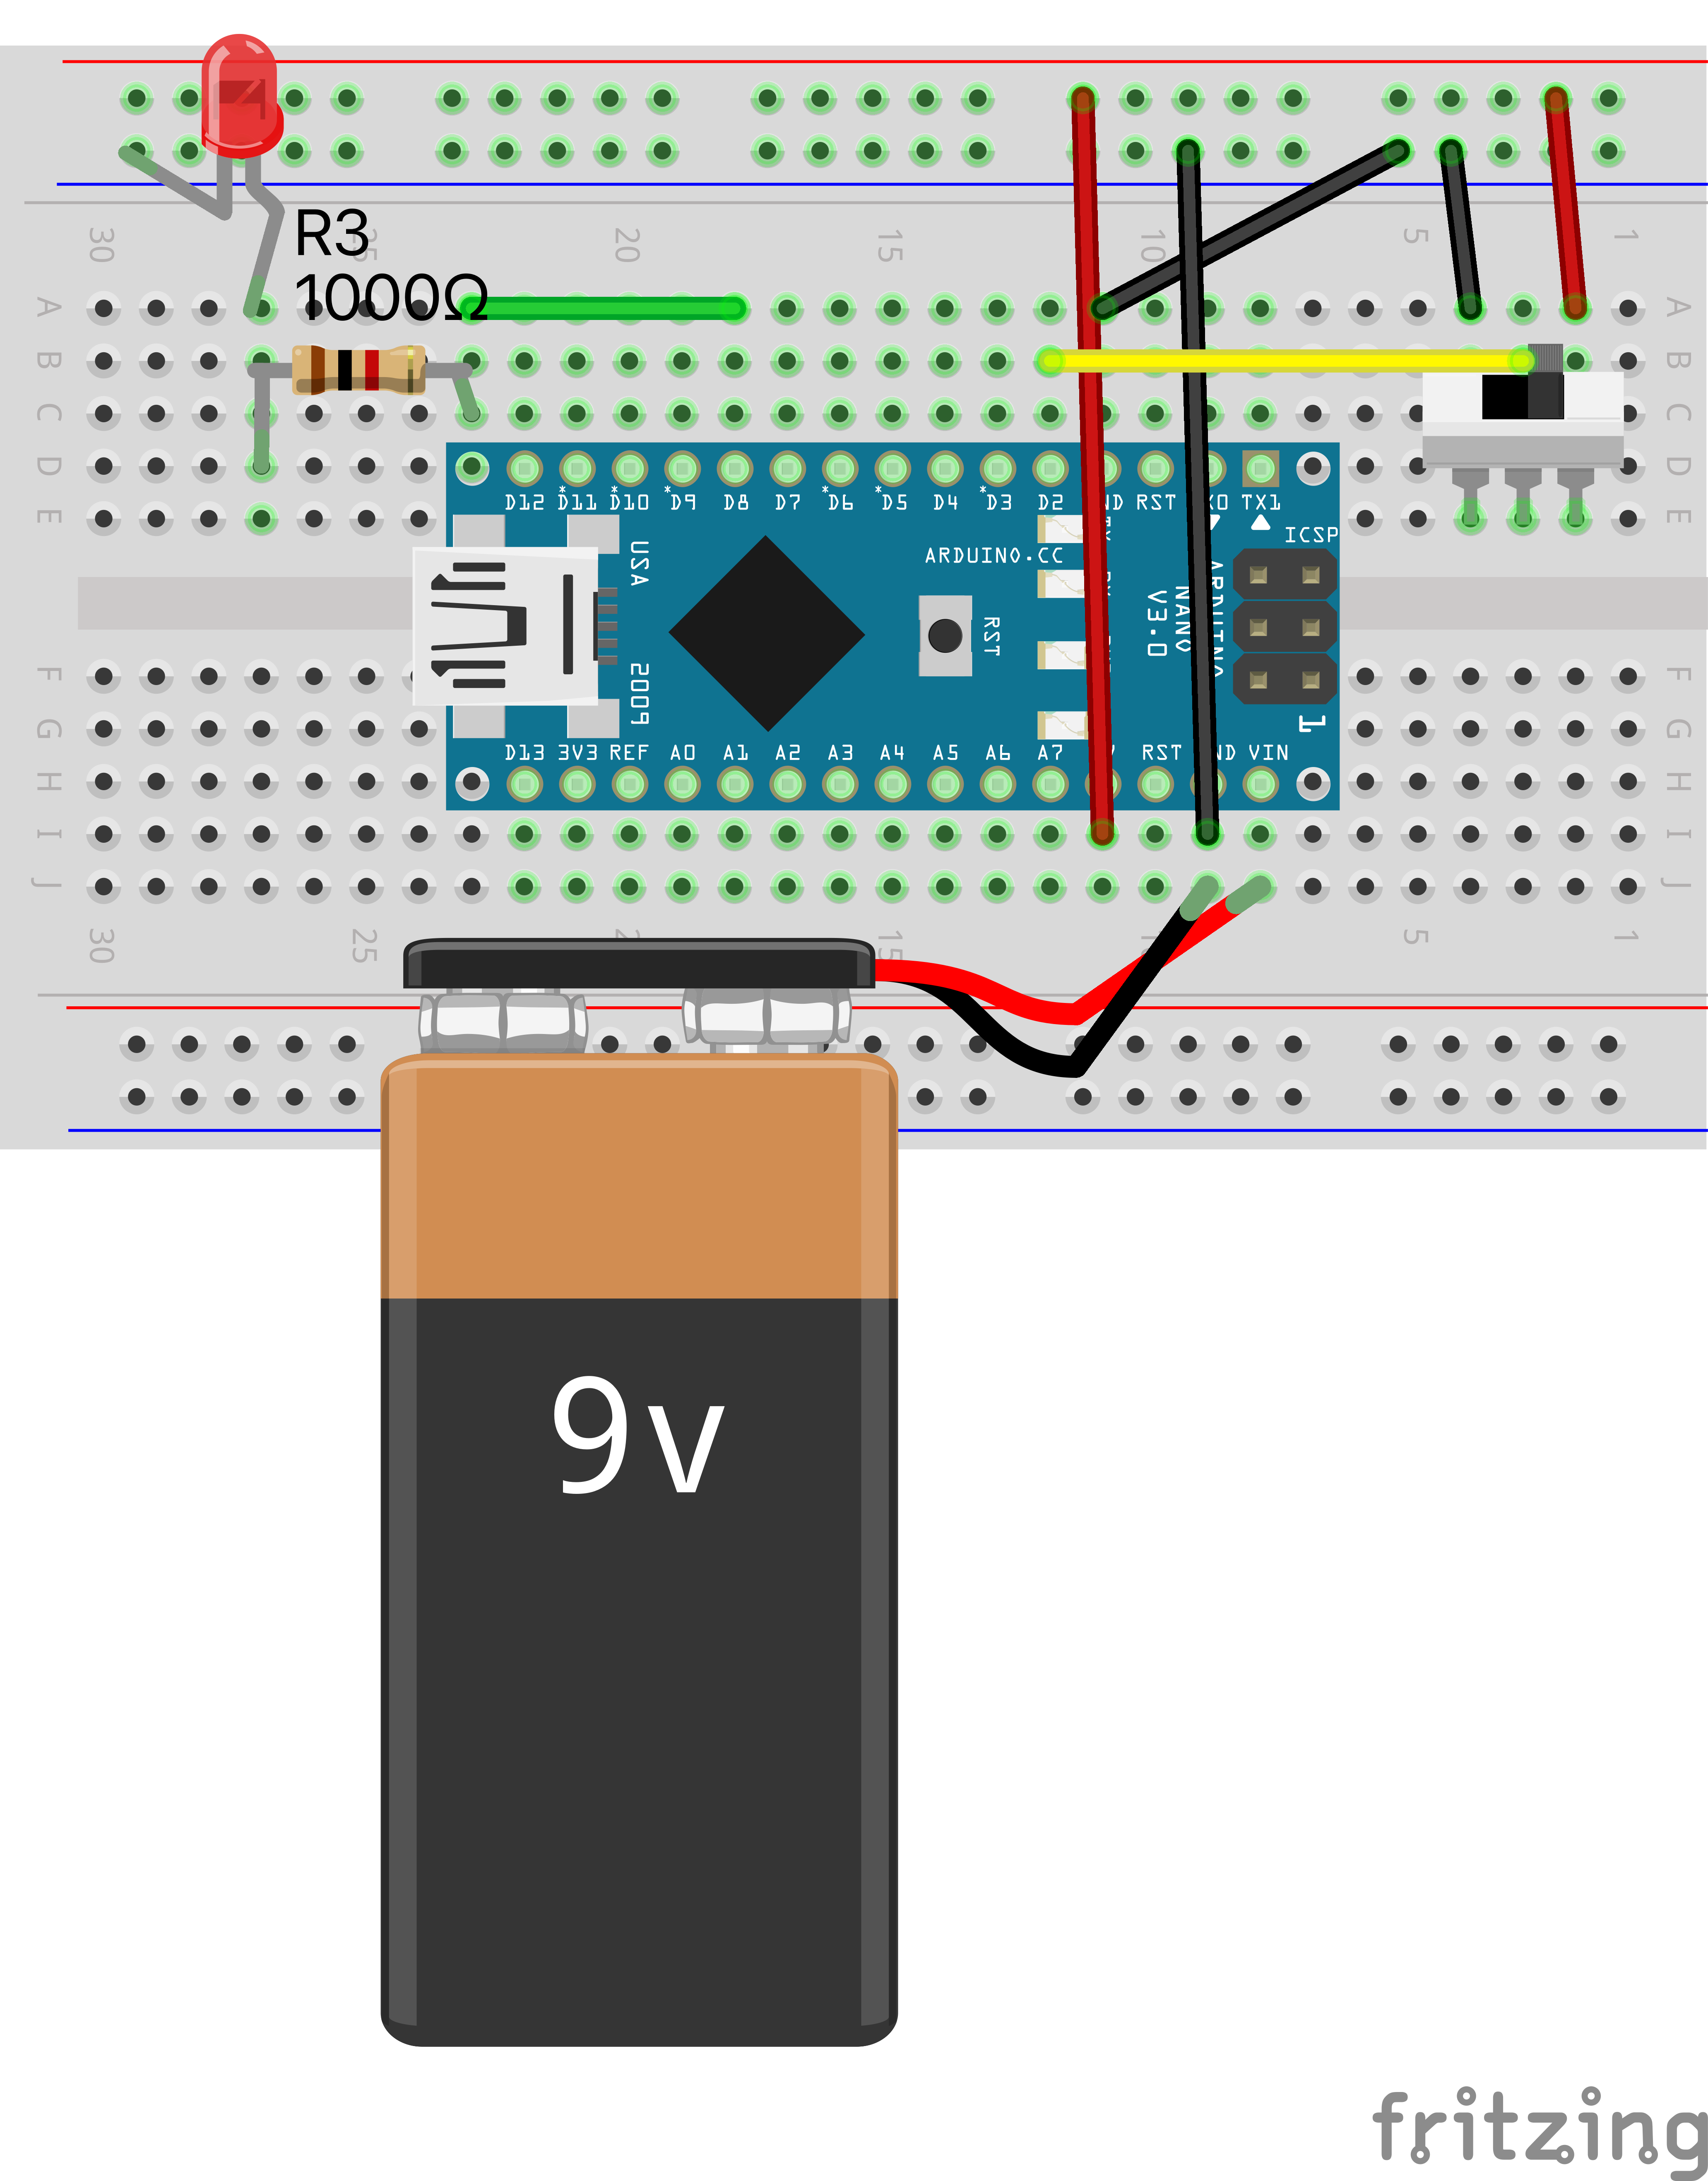
\includegraphics[width=0.8\textwidth]{led_switch_nano_bb.png}
\end{figure}
\newpage

\section*{Push Button Control}
\begin{minipage}{\textwidth}
Connect a push button to \texttt{pin 7}. Connect an LED to \texttt{pin 11}. Controls an LED with the button.
\end{minipage}
\begin{figure}[h!]
\centering
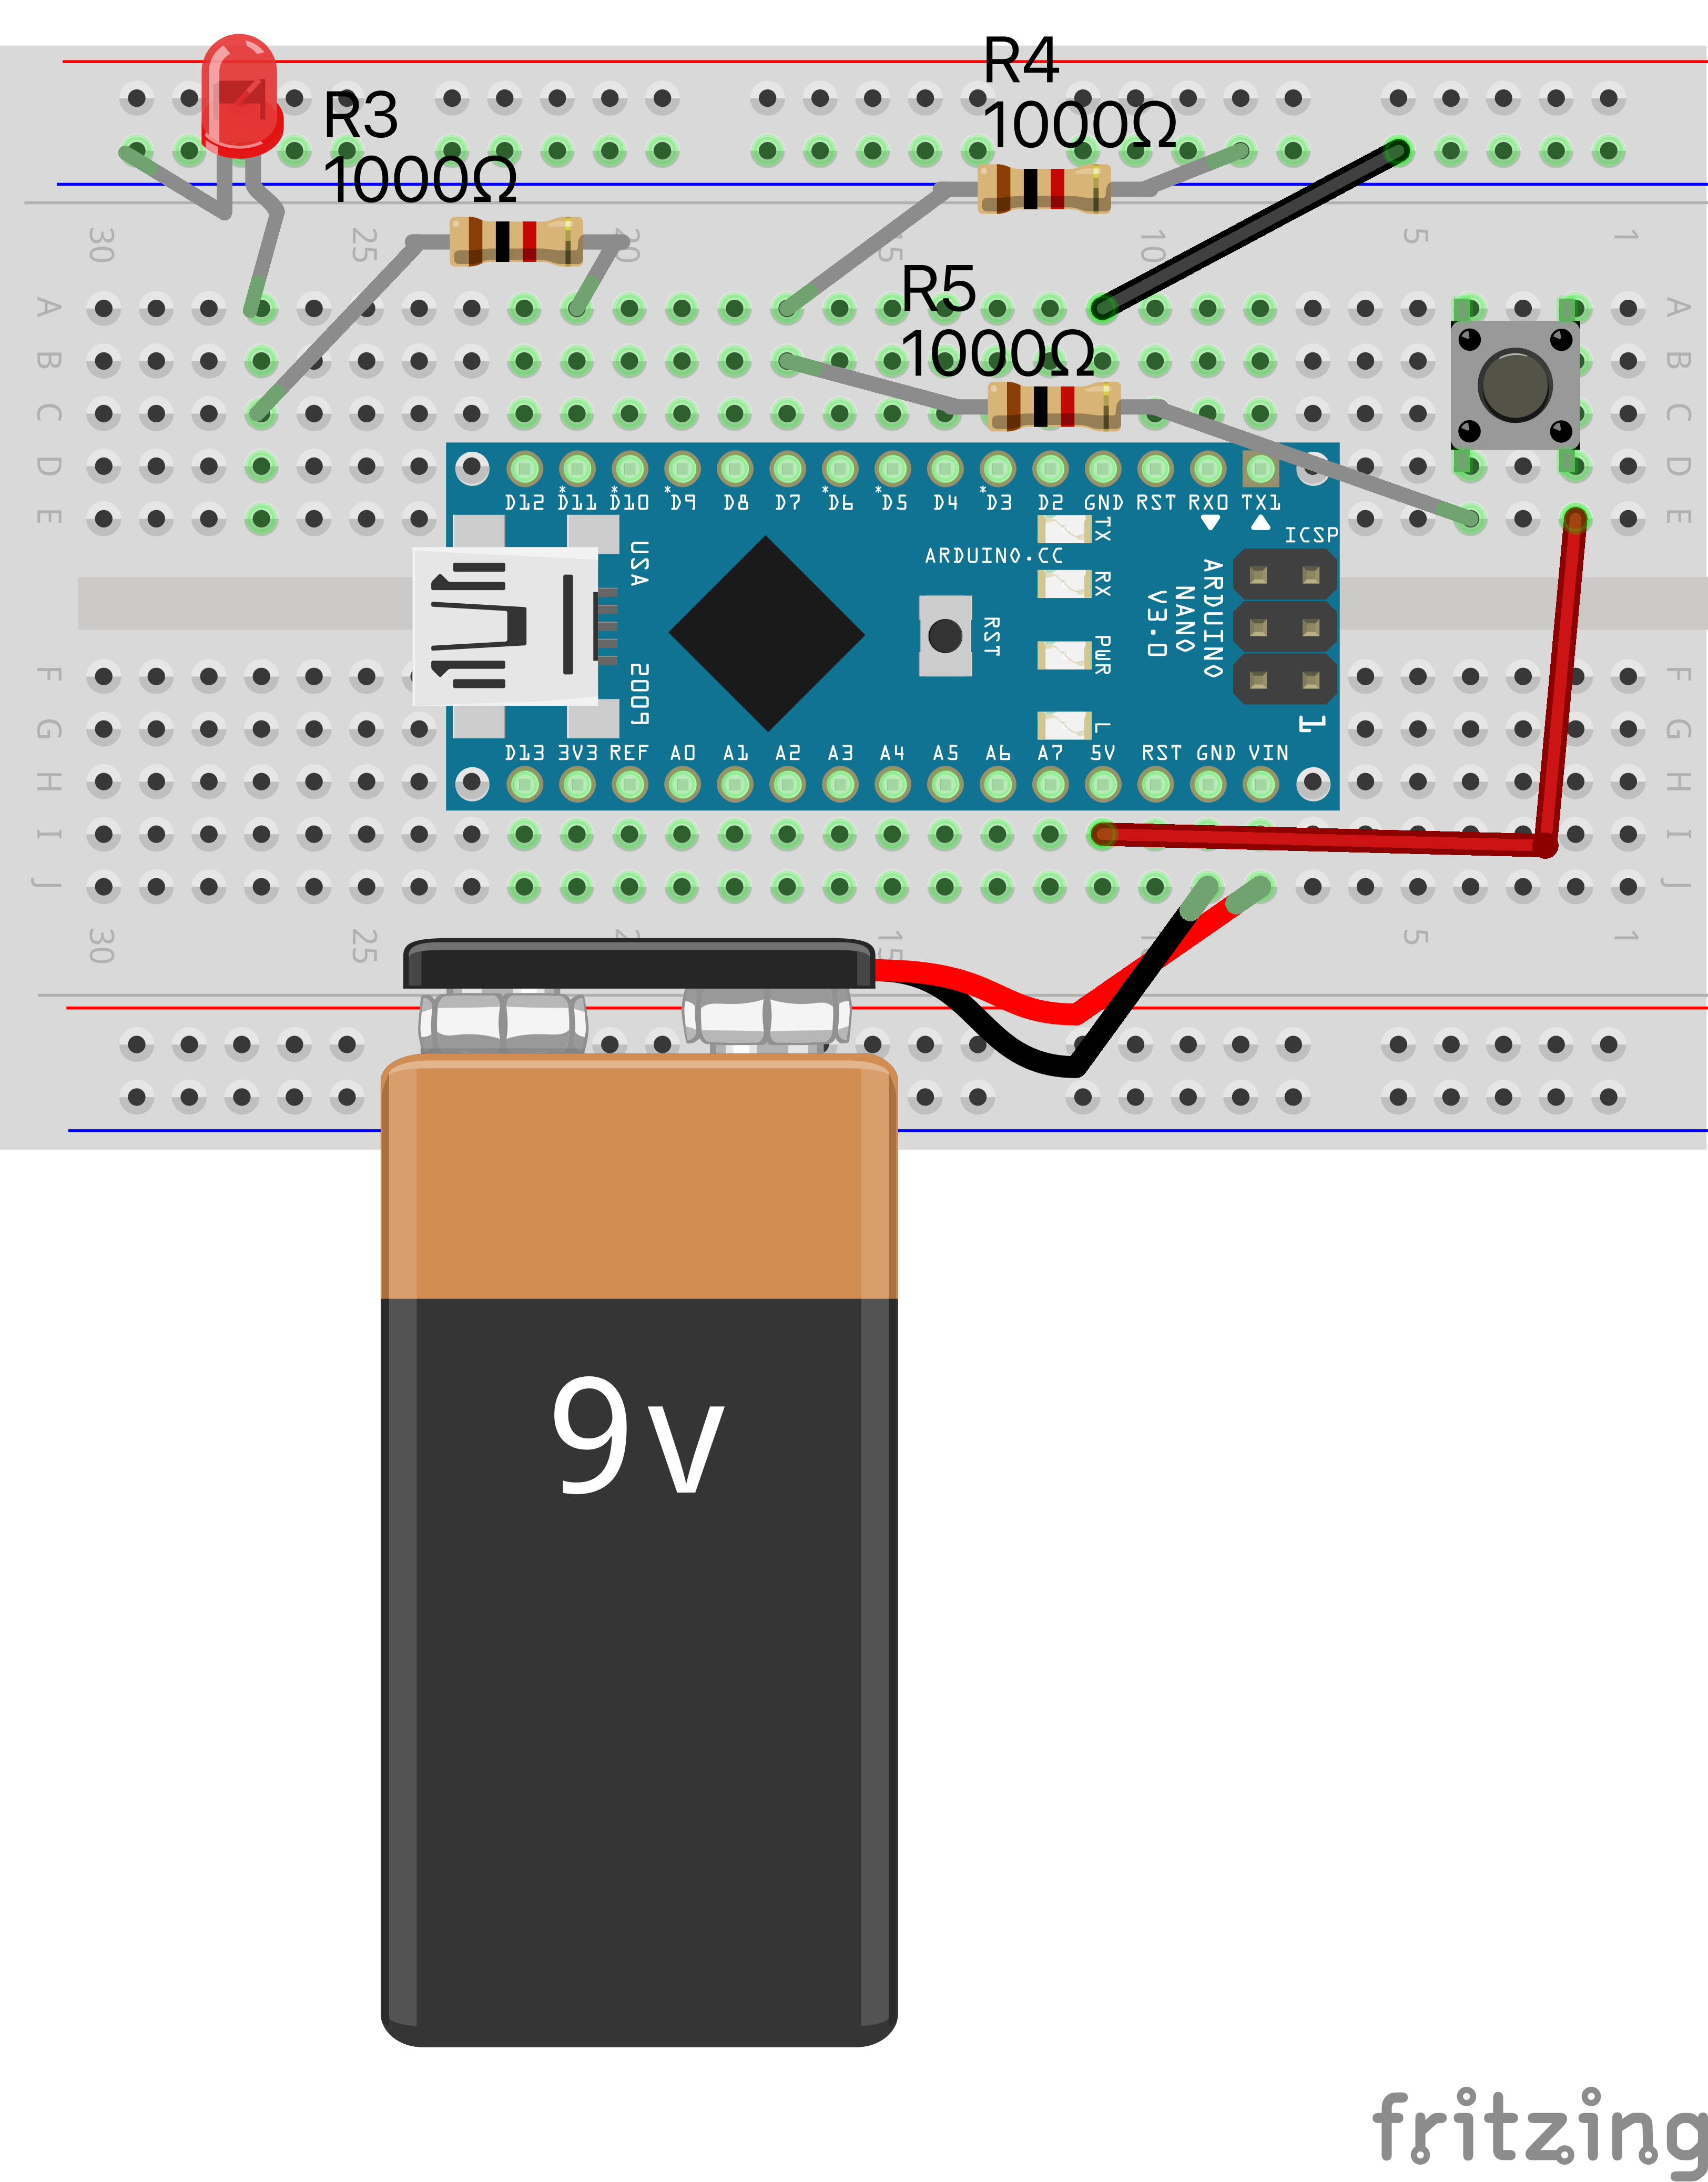
\includegraphics[width=0.8\textwidth]{button_nano_bb.png}
\end{figure}
\newpage

\section*{Photoresistor Control}
\begin{minipage}{\textwidth}
Connect a photoresistor to \texttt{A1}. Connect an LED to \texttt{pin 4}. Turns on an LED based on light levels near photoresistor.
\end{minipage}
\begin{figure}[h!]
\centering
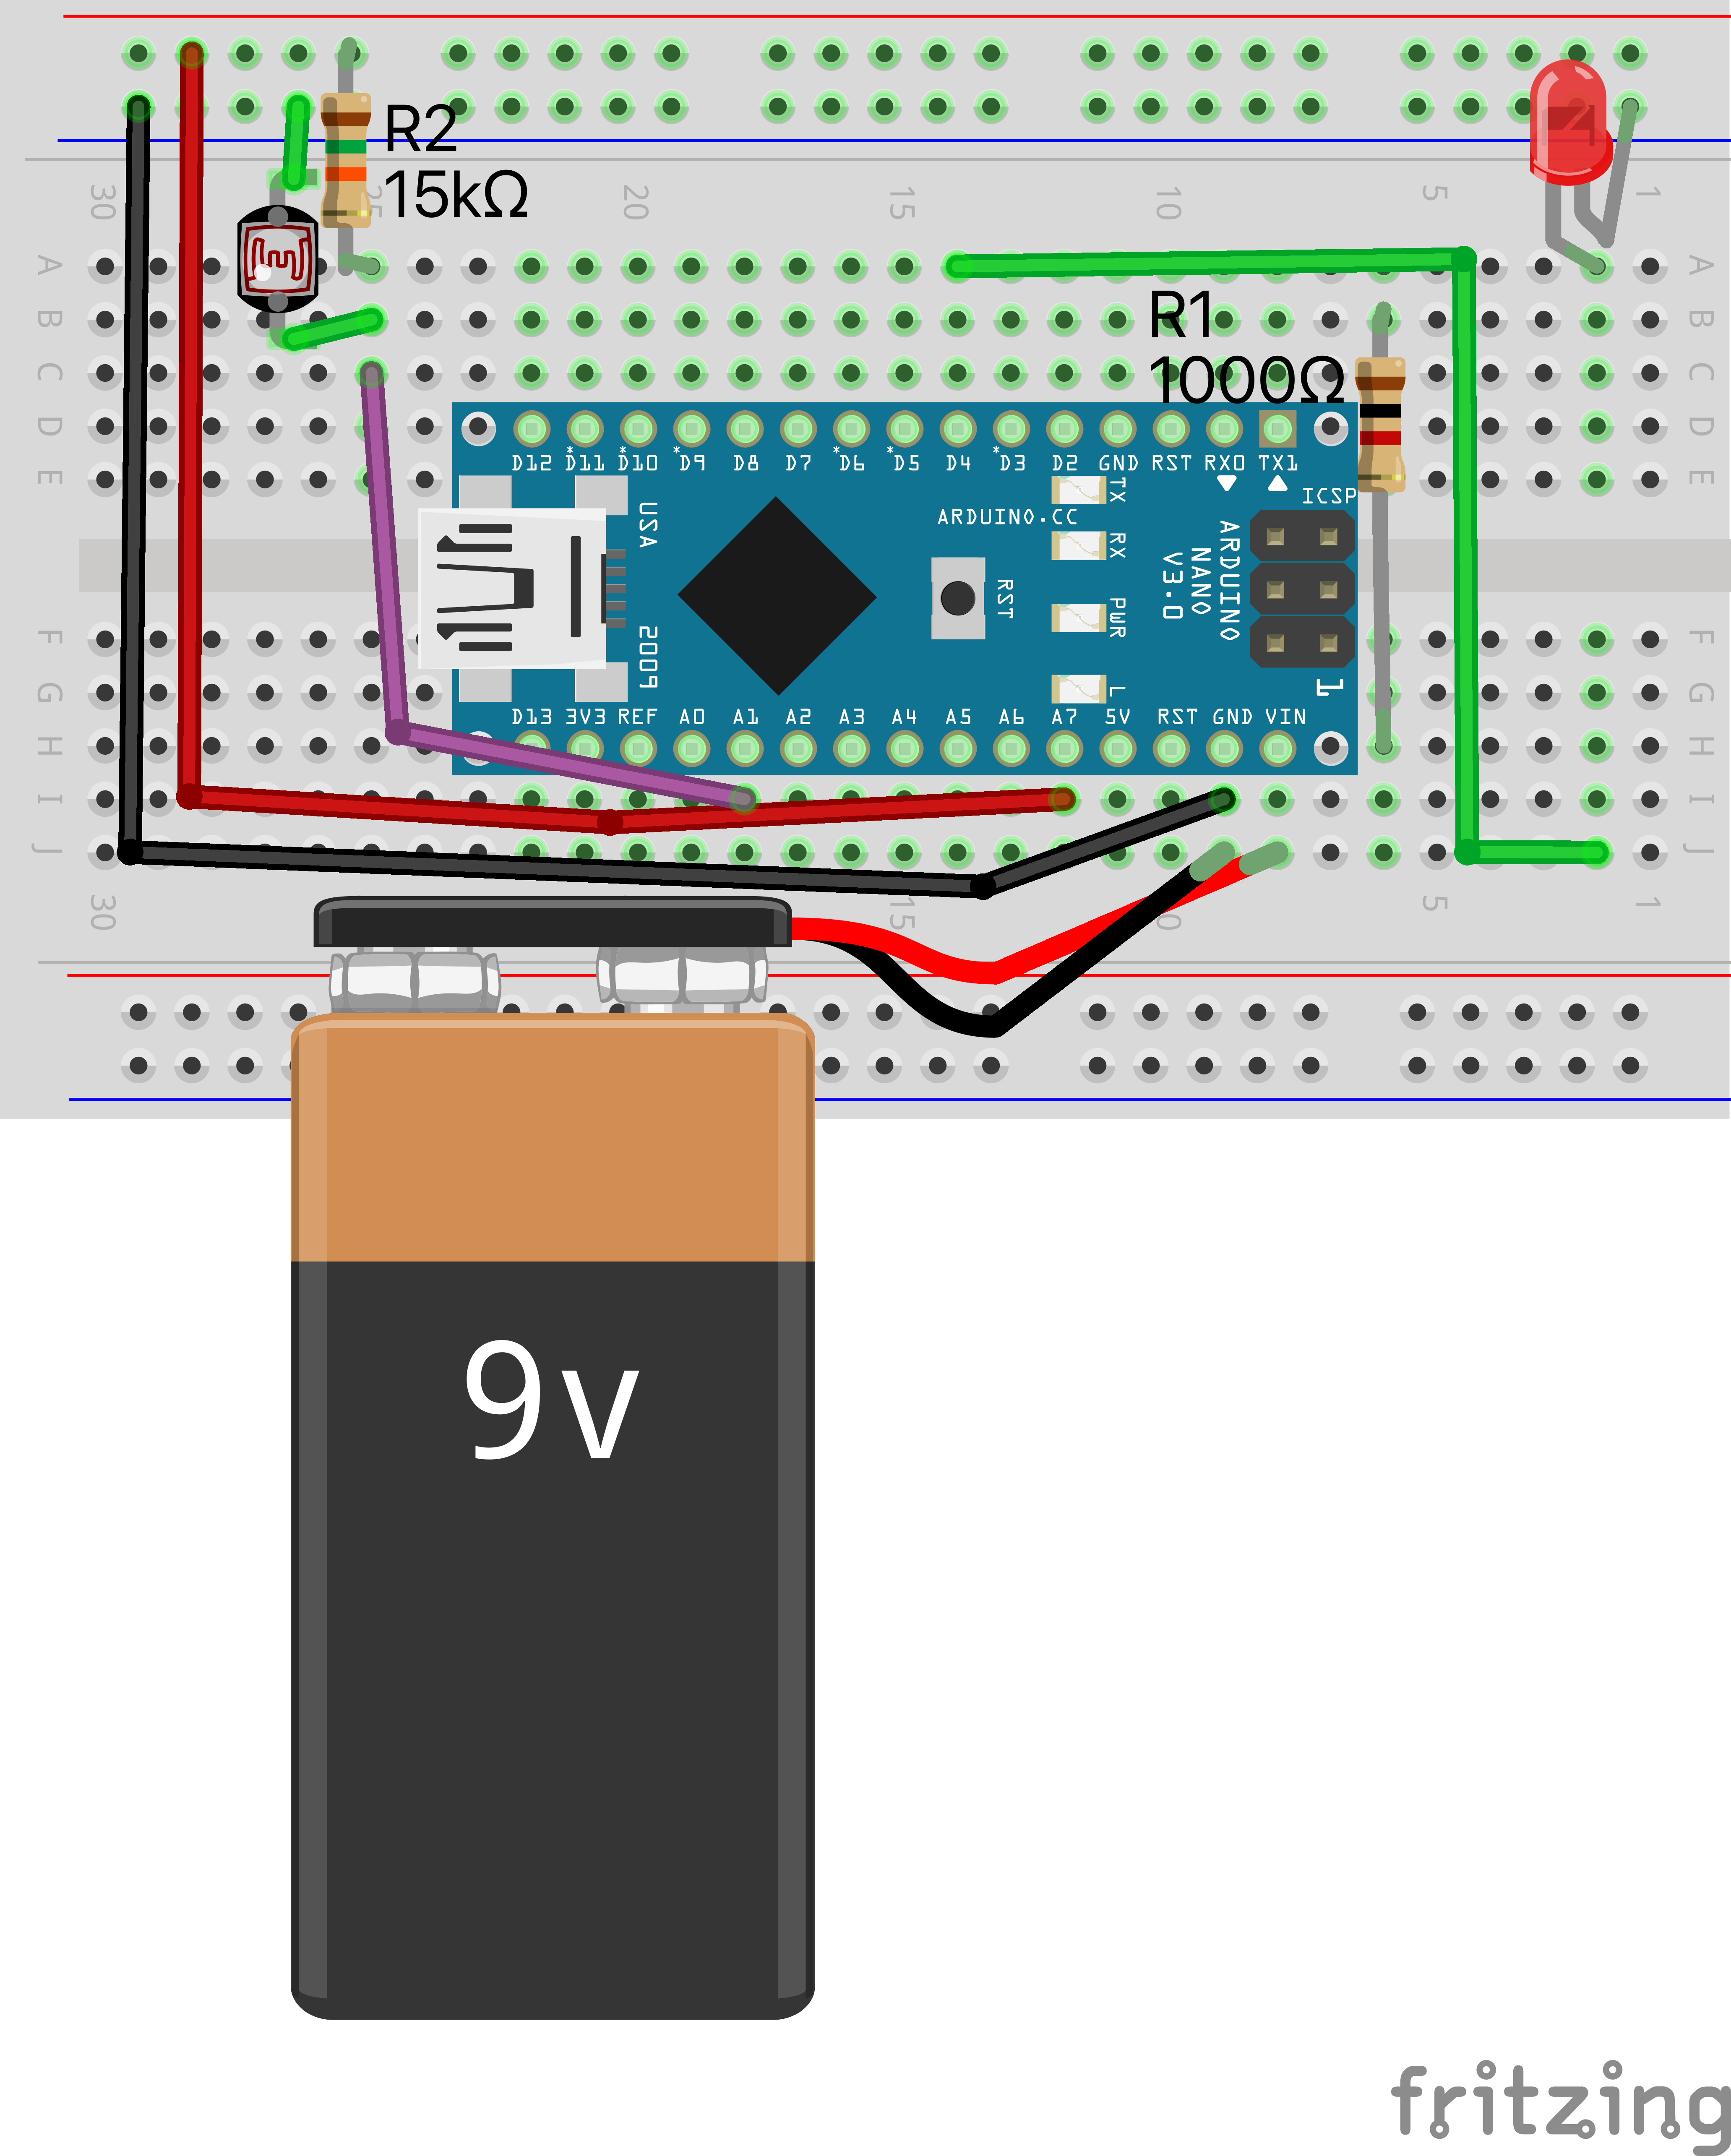
\includegraphics[width=0.8\textwidth]{photoresistor_nano_bb.png}
\end{figure}
\newpage

\section*{Potentiometer Control}
\begin{minipage}{\textwidth}
Connect a potentiometer to \texttt{A0}. Connect an LED to \texttt{pin 10}. Adjusts LED brightness with the potentiometer.
\end{minipage}
\begin{figure}[h!]
\centering
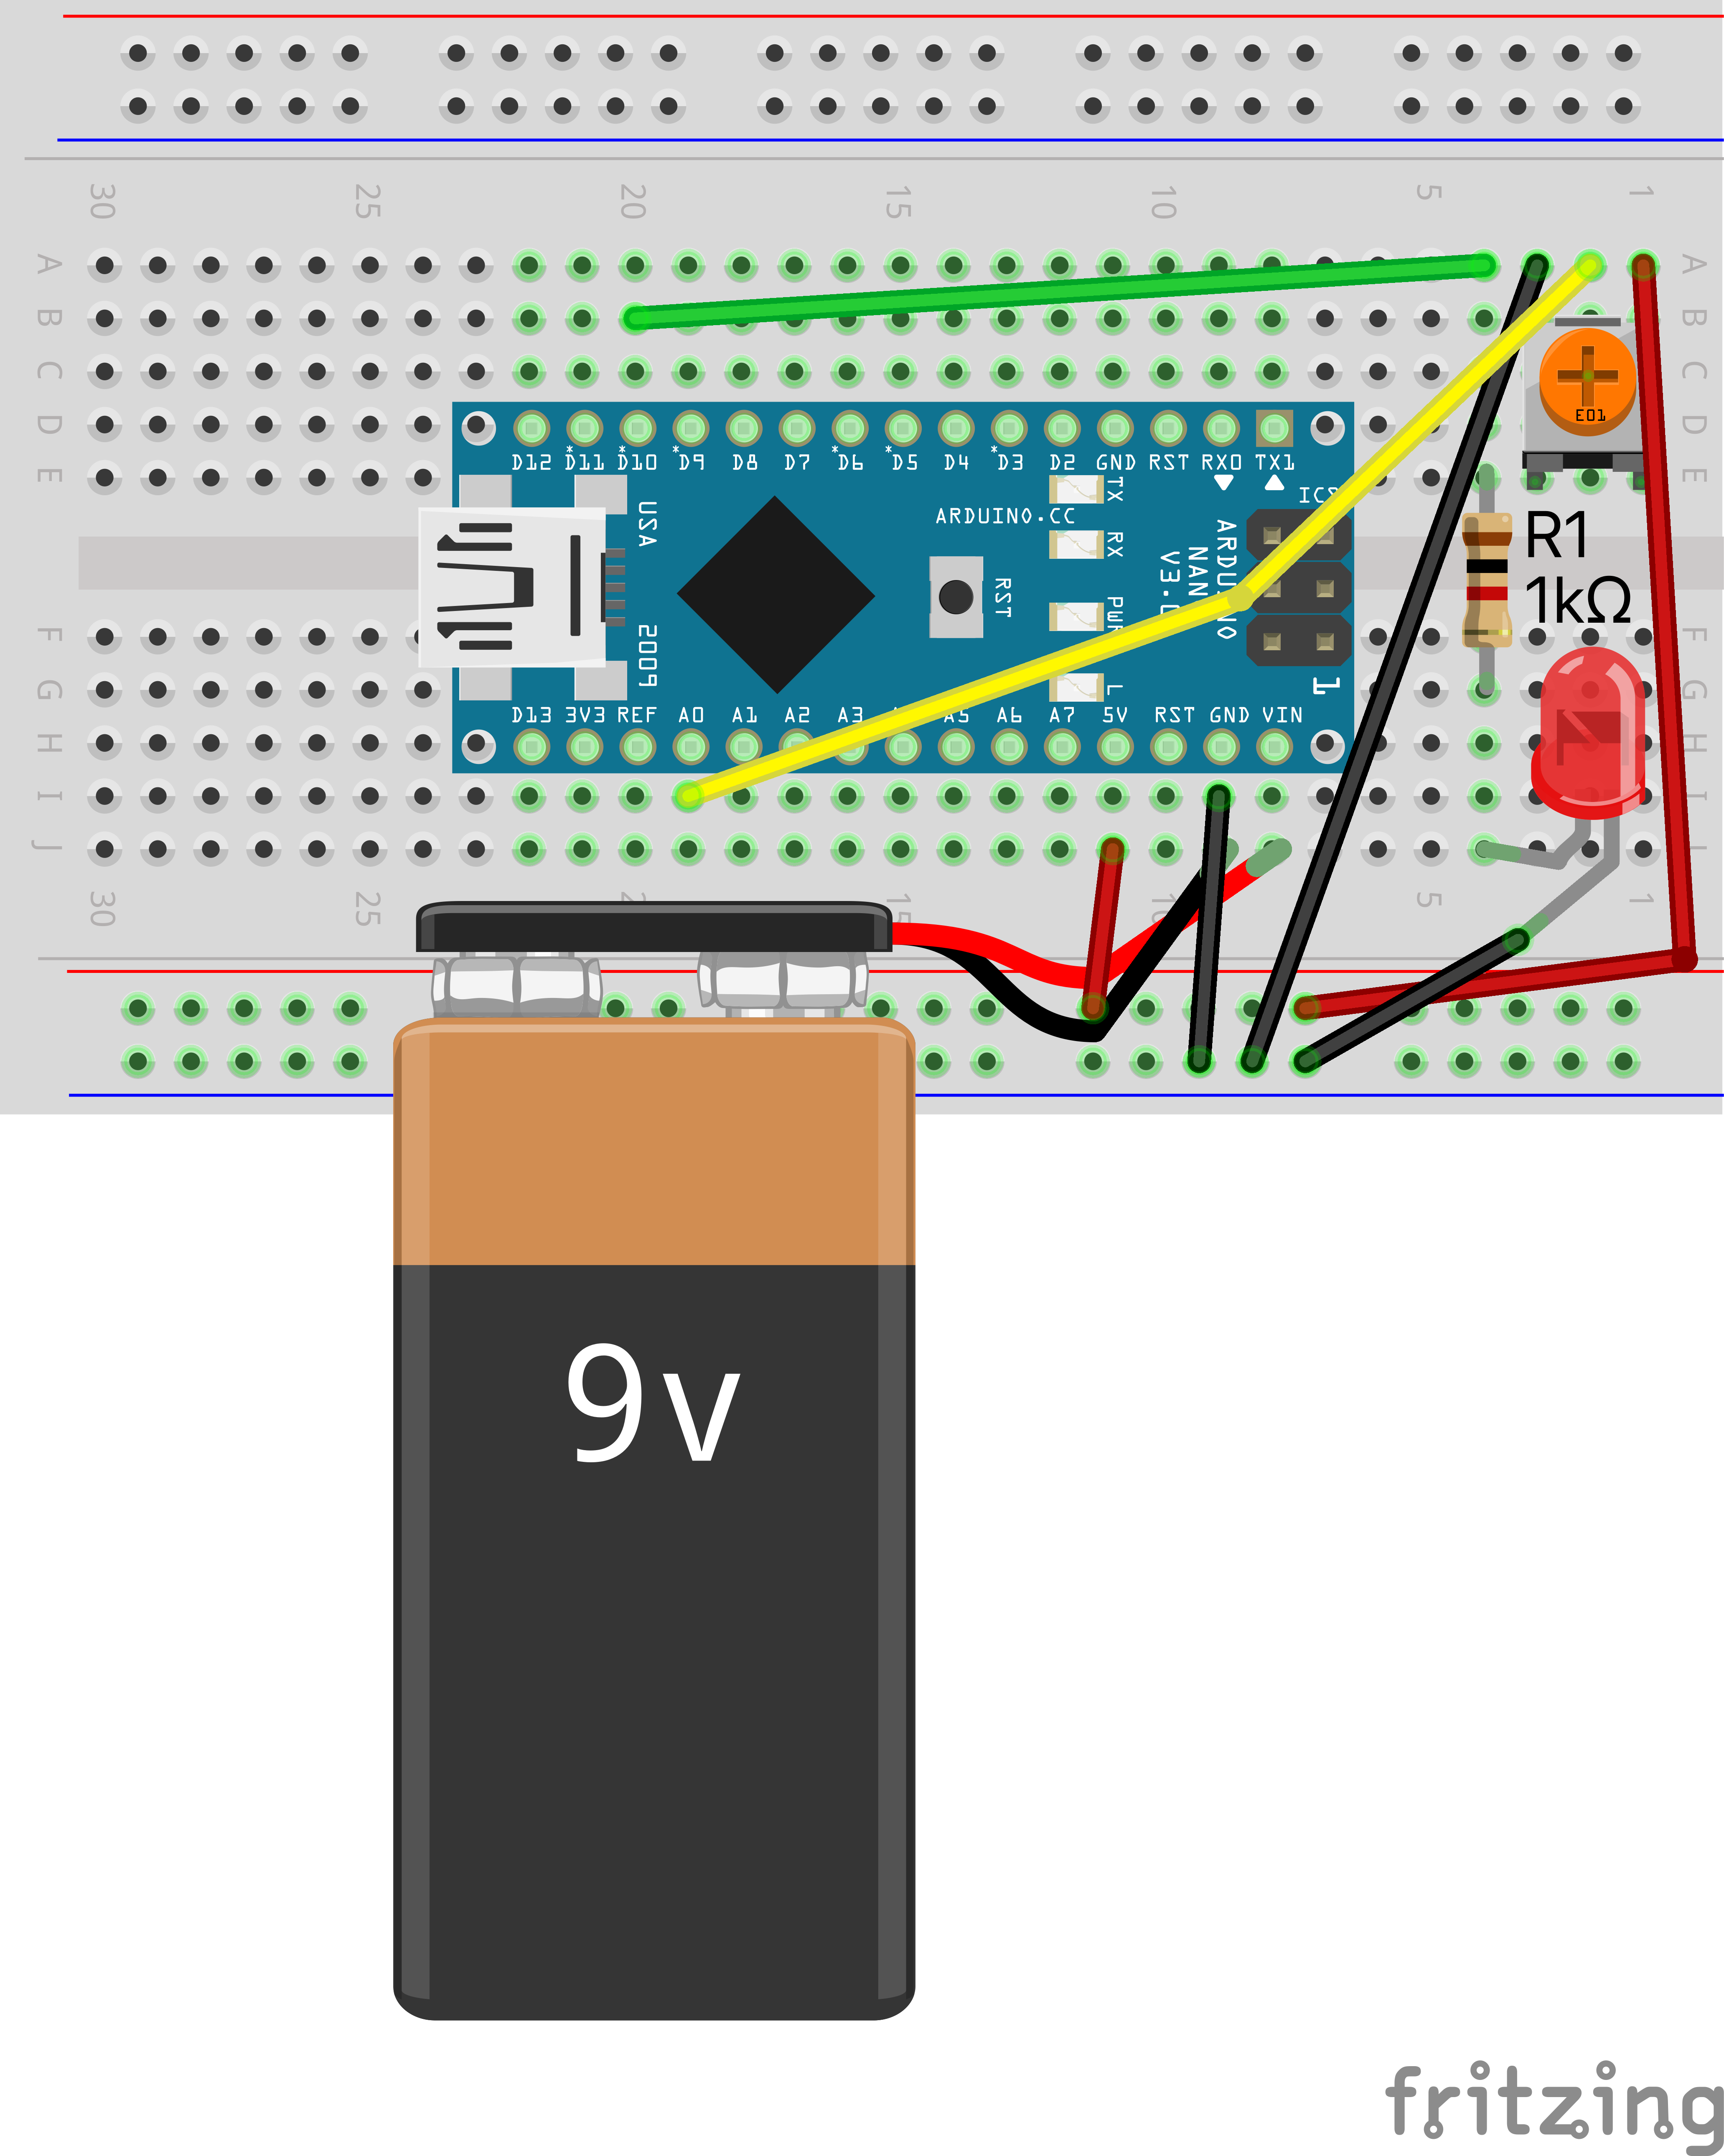
\includegraphics[width=0.8\textwidth]{potent_nano_bb.png}
\end{figure}

\end{document}
